%----------------------------------------------------------------------------------------
%    PACKAGES AND THEMES
%----------------------------------------------------------------------------------------

\documentclass[10pt,aspectratio=169,xcolor=dvipsnames]{beamer}
\usetheme{SimplePlus}

% Show only the section title on section-divider frames.
\setbeamertemplate{section page}{
    \begin{centering}
        \begin{beamercolorbox}[sep=12pt,center]{section title}
            \usebeamerfont{section title}\insertsectionhead\par
        \end{beamercolorbox}
    \end{centering}
}

\usepackage{lmodern}
\usepackage{natbib}
\renewcommand{\bibsection}{}
\usepackage{hyperref}
\usepackage{graphicx} % Allows including images
\usepackage{booktabs} % Allows the use of \toprule, \midrule and \bottomrule in tables
\input{math_commands.tex}

%----------------------------------------------------------------------------------------
%    TITLE PAGE
%----------------------------------------------------------------------------------------

\title{Decision-Focused Learning via Tangent-Space Projection of Prediction Error}
\subtitle{ICML 2026 \texorpdfstring{\citep{lee2026decisionfocusedlearningtangentspaceprojection}}{(Lee et al., 2026)}}

\author{Junhyeong Lee, Sangjin Jin, Yongjae Lee }

\institute
{
    Department of Industrial Engineering\\
    Ulsan National Institute of Science and Technology, Ulsan, South Korea.
}
\date{\today} % Date, can be changed to a custom date

%----------------------------------------------------------------------------------------
%    PRESENTATION SLIDES
%----------------------------------------------------------------------------------------

\begin{document}

\begin{frame}
    % Print the title page as the first slide
    \titlepage
\end{frame}

\begin{frame}{Overview}
    % Throughout your presentation, if you choose to use \section{} and \subsection{} commands, these will automatically be printed on this slide as an overview of your presentation
    \tableofcontents
\end{frame}

%------------------------------------------------
\section{Regret Gradient via Tangent-Space  Projection}
%------------------------------------------------

\begin{frame}[plain,noframenumbering]
    \sectionpage
\end{frame}

\begin{frame}{Problem Setup}
    Given contextual $\vx \in \R^d$, predict cost vector $\hat{\vc} = f_\vtheta(\vx) \in \R^n$ to estimate $\vc$. Given $\hat{\vc}$, consider convex problem:
    \begin{equation}
        \begin{aligned}
            & \vz^*(\hat{\vc})  \in \arg\min_{\vz \in \R^n} \{ \phi(\vz) + \hat{\vc}^\top \vz \}\\
            & \text{s.t.}\quad \mA_{p \times n} \vz = \vb ,\quad
             \mG_{m \times n} \vz \leq \vh.
        \end{aligned}
    \end{equation}

    DFL defines regret under real cost vector $\vc$ as:
    \begin{equation}
        R(\hat{\vc}; \vc) = \underbrace{[\phi(\vz^*(\hat{\vc})) + \vc^\top \vz^*(\hat{\vc})]}_{\text{predicted cost}} - \underbrace{[\phi(\vz^*(\vc)) + \vc^\top \vz^*(\vc)]}_{\text{optimal cost}}.
    \end{equation}

    Training $f_\vtheta$ requires gradient $\nabla_\vtheta R(\hat{\vc}; \vc)$ by
    \begin{equation}
        \frac{\mathrm{d} R(\hat{\vc}; \vc)}{\mathrm{d} \vtheta} = \frac{\partial R}{\partial \vz^*} \frac{\partial \vz^*}{\partial \hat{\vc}} \frac{\partial \hat{\vc}}{\partial \vtheta}.
    \end{equation}
    And the gradient w.r.t. $\hat{\vc}$ is
    \begin{equation}
        \frac{\partial R}{\partial \hat{\vc}} = \left( \frac{\partial \vz^*}{\partial \hat{\vc}} \right)^\top \left( \nabla_{\vz^*} \phi(\vz^*) + \vc \right).
    \end{equation}


\end{frame}

\begin{frame}{Active Set and Local Regularity}

    Main problem: active set ($\mathcal{A}(\hat{\vc}):=\{i \in [m] : \vg_i^\top \vz^*(\hat{\vc}) = \evh_i\}$) may change and thus $\hat{\vc} \mapsto \vz^*(\hat{\vc})$ may be non-smooth.
    \begin{block}{General framework (notations not consistent)}
       Consider $\vy^*(\vx) = \arg\min_{\vy \in \mathcal{Y}} g(\vx,\vy)$, $\vx$ may be viewed as a parameter.
       \begin{itemize}
            \item If $\mathcal{Y} = \R^n$ and $g$ is smooth and convex, then optimal solution $\vy^*(\vx)$ is given by $\nabla_{\vy} g(\vx,\vy^*(\vx)) = 0$. Then, by implicit function theorem, $\vy^*(\vx)$ is smooth when $\nabla^2_{\vy\vy} g(\vx,\vy^*(\vx))$ is non-singular.
            \item But if constrained (e.g. $\mathcal{Y} = \{\vy : \mG\vy \leq \vh\}$), then the optimality condition becoems $0 \in \nabla_{\vy} g(\vx,\vy^*(\vx)) + \mathcal{N}_{\mathcal{Y}}(\vy^*(\vx))$, where $\mathcal{N}_{\mathcal{Y}}(\vy)$ is the normal cone of $\mathcal{Y}$ at $\vy$.
            \item Therefore, when $\vx$ changes, the optimal solution $\vy^*(\vx)$ may change, shifting from one face of $\mathcal{Y}$ to another, and thus the active set may change. In short, $\vx \mapsto \mathcal{A}(\vx) \mapsto \vy^*(\vx)$, and $\mathcal{A}(\vx)$ may be discrete.
            \item Yet within each active set, $\vy^*(\vx)$ is smooth, thus it is piecewise smooth.
       \end{itemize}


    \end{block}


\end{frame}

\begin{frame}[allowframebreaks]{Appendix: Normal Cone}
    \begin{columns}[T,onlytextwidth]
        \begin{column}{0.7\textwidth}
            \textbf{Definition (Normal Cone).} For a closed convex set
            $\mathcal{Y} \subseteq \R^n$ and $\vy \in \mathcal{Y}$, the normal
            cone of $\mathcal{Y}$ at $\vy$ is defined as $\mathcal{N}_{\mathcal{Y}}(\vy) := \{\vv \in \R^n : \vv^\top (\vy' - \vy) \leq 0,\ \forall \vy' \in \mathcal{Y}\}$.
            \begin{itemize}
                \item  Tl;dr: vectors that point outward of $\mathcal{Y}$ at ref $\vy$.
                \item For polyhedral set $\mathcal{Y} = \{\vy : \mG\vy \leq \vh\}$, the normal cone is
                {\scriptsize
                \[
                \mathcal{N}_{\mathcal{Y}}(\vy) = \left\{\sum_{i \in \mathcal{A}(\vy)} \lambda_i \vg_i : \lambda_i \geq 0\right\}:=\cone\left\{\vg_i : i \in \mathcal{A}(\vy)\right\}
                \]}
                where $\mathcal{A}(\vy) := \{i : \vg_i^\top \vy = \evh_i\}$ is the active set at $\vy$, $\vg_i^\top$ is the $i$-th row of $\mG$, and $\cone\{S\}$ is the conic hull of $S$.
            \end{itemize}

        Thus, for such constrained problem, the optimality condition is $-\nabla_{\vy} g(\vx,\vy^*(\vx)) \in \mathcal{N}_{\mathcal{Y}}(\vy^*(\vx))$, i.e., the descent motion can be blocked by the the combination of active constraints (\emph{which is exactly the more general form of KKT condition}).

        \end{column}
        \begin{column}{0.27\textwidth}
            \centering
            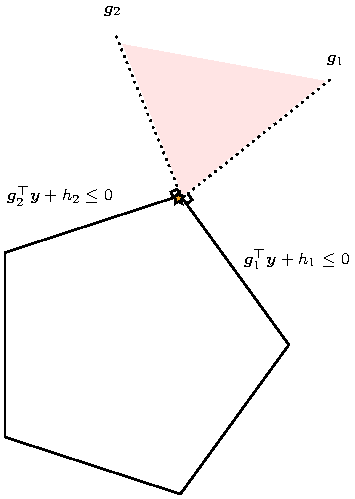
\includegraphics[width=0.9\linewidth]{output/pdf/normal_cone.pdf}
        \end{column}
    \end{columns}

    \break

    In a more convex analysis perspective, consider extended value indicator $\delta_{\mathcal{Y}}(\vy) = 0$ if $\vy \in \mathcal{Y}$, $+\infty$ otherwise.
    Then $\min_{\vy\in \mathcal{Y}} g(\vy) = \min_{\vy \in \R^n} \{g(\vy) + \delta_{\mathcal{Y}}(\vy)\} := \min_{\vy \in \R^n} F(\vy)$.


    \begin{block}{\small\textbf{Fact:} $\partial \delta_{\mathcal{Y}}(\vy) = \mathcal{N}_{\mathcal{Y}}(\vy)$}
        Proof. By subdifferential $\partial \delta_{\mathcal{Y}}(\vy) = \{\vv : \delta_{\mathcal{Y}}(\vy') \geq \delta_{\mathcal{Y}}(\vy) + \vv^\top (\vy' - \vy),\ \forall \vy'\}$.
        \[
            \begin{array}{c|c|c|c|c}
            \text{Case}
            & \delta_{\mathcal{Y}}(\vy)
            & \delta_{\mathcal{Y}}(\vy')
            & \text{Subgradient inequality}
            & \text{Consequence}
            \\
            \hline
            \vy\in \mathcal{Y},\ \vy'\in \mathcal{Y}
            & 0
            & 0
            & 0\ge \vv^\top(\vy'-\vy)
            & \boxed{\vv^\top(\vy'-\vy)\le 0}
            \\[4pt]

            \vy\in \mathcal{Y},\ \vy'\notin \mathcal{Y}
            & 0
            & +\infty
            & +\infty\ge \vv^\top(\vy'-\vy)
            & \text{Automatically satisfied}
            \\[4pt]

            \vy\notin \mathcal{Y},\ \vy'\in \mathcal{Y}
            & +\infty
            & 0
            & 0\ge +\infty
            & \text{Impossible}
            \\[4pt]

            \vy\notin \mathcal{Y},\ \vy'\notin \mathcal{Y}
            & +\infty
            & +\infty
            & +\infty\ge +\infty
            & \text{No additional restriction}
            \end{array}
        \]
        And the only non-trivial case is exactly the definition of normal cone.
    \end{block}
    Thus, the optimality condition can be written as $0 \in \nabla_{\vy} g(\vy^*) + \partial \delta_{\mathcal{Y}}(\vy^*) = \partial F(\vy^*)$.
\end{frame}

\begin{frame}[allowframebreaks]{Active set and Local Regularity (cont.)}
    Back to the original problem.

    \vspace{1em}

     Given $\hat{\vc}$, let $\mathcal{A}(\hat{\vc}) := \{i: (\mG \vz^*(\hat{\vc}))_i = \evh_i\}$ be the active set at $\vz^*(\hat{\vc})$. Define the substack of the active constraint matrix
    $$
    \mJ(\hat{\vc}) := \begin{bmatrix}
        \mA\\
        \mG_{\mathcal{A}(\hat{\vc})}
    \end{bmatrix} \in \R^{k\times n},\quad k = p + |\mathcal{A}(\hat{\vc})|.
    $$


    This paper focuses on each neighbourhood, where $\mathcal{A}(\hat{\vc})$ is unchanged, i.e., $\mathcal{A}(\hat{\vc}) = \mathcal{A}(\hat{\vc} + d\hat{\vc})$ for sufficiently small perturbation $d\hat{\vc}$. Thus, $\mJ(\hat{\vc}) = \mJ(\hat{\vc} + d\hat{\vc}) := \mJ$ is fixed, and the solution map $\vz^*(\hat{\vc})$ is smooth w.r.t. $\hat{\vc}$.


    \begin{block}{\small Note on $\mJ$}
        \begin{itemize}
            \item Since all constraints are linear, $\mJ(\hat{\vc})$ is also the Jacobian of the active constraints at $\vz^*(\hat{\vc})$.
            \item $\mJ: \R^n \to \R^k$ is a linear map from decision space to active constraint space.
            \item $\mJ d\vz$ can be viewed as: if $\vz$ has a tiny perturbation $d\vz$, then $\mJ d\vz$ is the corresponding change of the active constraint values on each row.
        \end{itemize}
    \end{block}

    \break

    To further ensure smothness within each region, it requires the following classical regularity conditions:
    \begin{itemize}
        \item $\mH = \nabla^2 \phi(\vz^*(\hat{\vc}))$ is positive definite.
        \item LICQ (linearly independent constraint qualification): $\mJ(\hat{\vc})$ is full row rank.
        \item Strict complementarity: For active inequality constraints $i \in \mathcal{A}$, the corresponding Lagrange multiplier $\evmu_i^* > 0$; for inactive constraints $i \notin \mathcal{A}$, $\evmu_i^* = 0$.
    \end{itemize}
    These assumptions ensure: solution map is locally unique, continuous, and active set is invariant under sufficiently small perturbation of $\hat{\vc}$.

\end{frame}

\begin{frame}[allowframebreaks]{Sensitivity via a Reduced KKT System}
    The origin KKT system is
    \begin{equation}
        \begin{aligned}
            \nabla \phi(\vz^*) + \mA^\top \vlambda^* + \mG^\top \vmu^* + \hat{\vc} &= 0\\
            \mA \vz^* = \vb, ~ \mG \vz^* \leq \vh , \vmu^* &\geq 0, \\~ \diag(\vmu^*) (\mG \vz^* - \vh) &= 0.
        \end{aligned}
    \end{equation}

    Under the regularity conditions, focusing on local neighbourhood of $\hat{\vc}$, the reduced KKT system is
    \begin{equation}\label{eq:reduced_kkt}
        \nabla \phi(\vz^*) + \hat{\vc} + \mJ^\top \vy^* = 0 , ~ \mJ \vz^* = \tilde{\vb},
    \end{equation}
    where
    \begin{equation}
        \mJ = \begin{bmatrix}
            \mA\\
            \mG_{\mathcal{A}(\hat{\vc})}
        \end{bmatrix},\quad
        \vy^* = \begin{bmatrix}
            \vlambda^*\\
            \vmu^*_{\mathcal{A}(\hat{\vc})}
        \end{bmatrix},\quad
        \tilde{\vb} = \begin{bmatrix}
            \vb\\
            \vh_{\mathcal{A}(\hat{\vc})}
        \end{bmatrix}.
    \end{equation}
    Form~\eqref{eq:reduced_kkt} into a linear system:
    \begin{equation}
        F(\vz, \vy, \hat{\vc}) = \begin{bmatrix}
            \nabla \phi(\vz) + \hat{\vc} + \mJ^\top \vy\\
            \mJ \vz - \tilde{\vb}
        \end{bmatrix} = 0.
    \end{equation}
    Taking the differential of $F$ w.r.t. $(\vz, \vy)$ and $\hat{\vc}$ gives the sensitivity of the solution w.r.t. $\hat{\vc}$:
    \begin{equation}\label{eq:reduced_kkt_linear}
        \boxed{
            \begin{bmatrix}
                \mH & \mJ^\top\\
                \mJ & 0
            \end{bmatrix}
            \begin{bmatrix}
                d\vz\\
                d\vy
            \end{bmatrix}
            =
            \begin{bmatrix}
                -d\hat{\vc}\\
                0
            \end{bmatrix}
        } \qquad \text{where } \mH = \nabla^2 \phi(\vz^*).
    \end{equation}

    \textbf{Now consider its geometric interpretation.}

    This equation is invertivle under the regularity conditions, and thus the first row gives $\mH d\vz + \mJ^\top d\vy = -d\hat{\vc}$.
    \begin{equation}\label{eq:dz_dy}
        \implies d\vz = -\mH^{-1} d\hat{\vc} - \mH^{-1} \mJ^\top d\vy.
    \end{equation}


    Plug this in $\mJ d\vz = 0$ gives $\mJ \mH^{-1} \mJ^\top d\vy = -\mJ \mH^{-1} d\hat{\vc}$, and thus $d\vy = -(\mJ \mH^{-1} \mJ^\top)^{-1} \mJ \mH^{-1} d\hat{\vc}$.

    Finally, plug $d\vy$ back to \eqref{eq:dz_dy} gives
    \begin{equation}\label{eq:dz_dhatc_final}
        d\vz = -\left( \mH^{-1} - \mH^{-1} \mJ^\top (\mJ \mH^{-1} \mJ^\top)^{-1} \mJ \mH^{-1} \right) d\hat{\vc} = -\mP_H d\hat{\vc}.
    \end{equation}
    \begin{equation}\label{eq:dz_dhatc}
        \boxed{\frac{\partial \vz^*}{\partial \hat{\vc}} = -\mP_H}
    \end{equation}

    \break

    In last page, we denote $\mP_H = \mH^{-1} - \mH^{-1} \mJ^\top (\mJ \mH^{-1} \mJ^\top)^{-1} \mJ \mH^{-1} := \mPi_H \mH^{-1}$, where
    \begin{equation}
        \boxed{\mPi_H := \mI - \mH^{-1} \mJ^\top (\mJ \mH^{-1} \mJ^\top)^{-1} \mJ}
    \end{equation}

    Mathematically, $\mPi_H$ is a projection matrix onto the kernel of $\mJ$ ($\ker(\mJ) := \{\vv : \mJ \vv = 0\}$), under $\mH$-orthogonal (i.e., by conisdering the inner product induced by $\langle \vu,\vv\rangle_{\mH} = \vu^\top \mH \vv$).

    \begin{block}{\small Understanding of $\mJ$, its kernel and range}
        \begin{itemize}
            \item Kernel of $\mJ$: $\ker(\mJ) = \{\vv : \mJ \vv = 0\} \subseteq \R^n$, i.e., all directions that do not change the active constraint values. This is exactly the meaning of the tangent space, and denote $\mathcal{T}_{\vz^*} := \ker(\mJ)$.
            \item Range of $\mJ$: $\range(\mJ) = \{\vu : \vu = \mJ \vv,~\vv \in \R^n\} \subseteq \R^k$, i.e., all possible changing values of the active constraints from decision perturbations. (But we don't really care).
            \item Range of $\mJ^\top (\R^k \to \R^n$): Recall the KKT \eqref{eq:reduced_kkt} $\nabla_{\vz^*} \phi(\vz^*) + \hat{\vc} + \mJ^\top \vy^* = 0$, $\vy^*$ is the Lagrange multiplier (as weights of active constraints' gradients), to balance the descent direction $-\nabla_{\vz^*} \phi(\vz^*) - \hat{\vc}$.

            \emph{Thus, if for arbitrary $\vy \in \R^k$, $\mJ^\top \vy$ is the linear combination of active constraints' gradients, i.e., the normal space of the tangent space. Denote $\mathcal{N}_{\vz^*} := \range(\mJ^\top)$.}

            As a matter of fact:
            \begin{equation}
                \range(\mJ^\top) = \ker(\mJ)^\perp = \mathcal{T}_{\vz^*}^\perp = \mathcal{N}_{\vz^*}.
            \end{equation}
        \end{itemize}
    \end{block}

    \break

    Recall $\mP_H = \mH^{-1} - \mH^{-1} \mJ^\top (\mJ \mH^{-1} \mJ^\top)^{-1} \mJ \mH^{-1} := \mPi_H \mH^{-1}$.

    \vspace{1em}

    Then revisit this $\mPi_H$: \emph{projection onto $\ker(\mJ)$ under $\mH$-orthogonal}. It means that, for any direction $\vv \in \R^n$, $\mPi_H \vv$ is the closest vector to $\vv$ in $\ker(\mJ)$ under the $\mH$-norm, and it will always be in the tangent space, not changing the active constraints' values.

    \break

    Recall that \eqref{eq:dz_dhatc_final}: $d\vz = -\mP_H d\hat{\vc} = -\mPi_H \mH^{-1} d\hat{\vc}$ (i.e.,$\mP_H: d\hat{\vc} \mapsto d\vz$). Then, the geometric interpretation of $\mP_H$ is:
    \begin{itemize}
        \item $\mPi_H$ is the projection of movement. Yet $d\hat{\vc}$ is the perturbation of the predicted cost, not the decision.
        \item If this problem is unconstrained, i.e., $\min_{\vz} \phi(\vz) + \hat{\vc}^\top \vz$, then $\nabla \phi(\vz^*) + \hat{\vc} = 0$, and thus $d\vz = - \nabla^2 \phi(\vz^*)^{-1} d\hat{\vc} = -\mH^{-1} d\hat{\vc}$. So first we know: $\mH^{-1} d\hat{\vc}$ maps the perturbation of predicted cost to the perturbation of decision.
        \item Then, given that there are active constraints, $\mPi_H$ projects the perturbation of decision onto the tangent space, to ensure that the active constraints' values are unchanged.
    \end{itemize}

    \break

    Then the paper shows that,
    \begin{equation}
        {\mJ \mP_H = 0 , \qquad \mP_H \mJ^\top = 0}.
    \end{equation}
    \begin{itemize}
        \item The first one is obvious, since $\mP_H$ projects onto $\ker(\mJ)$, thus $\mJ \mP_H = 0$. \emph{Any primal movement caused by the perturbation of predicted cost will not change the active constraints' values (in first-order approximation).}
        \item The second is less obvious.

        Consider a special cost perturbation $d\hat{\vc} \in \range(\mJ^\top)$, i.e., $d\hat{\vc} = \mJ^\top d\vy$ for some $d\vy$. Then the KKT (\eqref{eq:reduced_kkt}) gives $\nabla \phi(\vz^*) + \hat{\vc} + \mJ^\top (\vy^* + d\vy) = 0$, thus the optimal solution does not change; we only need to adjust the Lagrange multiplier $\vy^*$ to balance the new cost perturbation. Thus, $d\vz = 0$.

        Meanwhile, \eqref{eq:dz_dhatc_final} gives $d\vz = -\mP_H d\hat{\vc} = -\mP_H \mJ^\top d\vy = 0$, thus $\mP_H \mJ^\top = 0$.

        \emph{Any cost perturbation in the normal space of the tangent space does not change the optimal solution.}
    \end{itemize}


\end{frame}

\begin{frame}[allowframebreaks]{Regret Gradient and the Projected Prediction Error}
    Recall that, our key is still to solve $\frac{\partial R}{\partial \hat{\vc}} = \left( \frac{\partial \vz^*}{\partial \hat{\vc}} \right)^\top \left( \nabla_{\vz^*} \phi(\vz^*) + \vc \right)$.
    \begin{itemize}
        \item The first term, $\frac{\partial \vz^*}{\partial \hat{\vc}} = -\mP_H$ (\eqref{eq:dz_dhatc}) measures how much decision $\vz^*$ changes w.r.t. predicted cost $\hat{\vc}$. Moreover, note that $\mP_H = \mP_H^\top$ is symmetric.
        \item The second term, from reduced KKT (\eqref{eq:reduced_kkt}), $\nabla_{\vz^*} \phi(\vz^*) + \hat{\vc} + \mJ^\top \vy^* = 0$, thus $\nabla_{\vz^*} \phi(\vz^*) + \vc = (\vc - \hat{\vc}) - \mJ^\top \vy^*$.
    \end{itemize}
    Plug in the two gives
    \begin{equation}
        \nabla_{\hat{\vc}} R(\hat{\vc}; \vc) = -\mP_H (\vc - \hat{\vc} - \mJ^\top \vy^*) = \mP_H (\hat{\vc} - \vc) + \underbrace{\mP_H \mJ^\top}_{=0} \vy^* = \mP_H (\hat{\vc} - \vc).
    \end{equation}
    Denote $\ve = \hat{\vc} - \vc$ as the prediction error, then the key formula, i.e. projected prediction error, is
    \begin{equation}\label{eq:regret_gradient}\boxed{
        \nabla_{\hat{\vc}} R(\hat{\vc}; \vc) = \mP_H \ve}
    \end{equation}

    Compared with MSE gradient $\nabla_{\hat{\vc}} \mathcal{L}_{\text{MSE}} = \hat{\vc} - \vc = \ve$, it implies: \emph{each direction of pred.error needs to be adjusted}.

    \break

    \begin{corollary}[Normal Filtering and Normal Invariance]
        Let $\mathcal{N} = \range(\mJ^\top)$ be the normal space of the tangent space $\mathcal{T}$. For any $\vdelta_N \in \mathcal{N}$,
        \begin{equation}\label{eq:normal_invariance}
            \mP_H \vdelta_N = 0 .
        \end{equation}
         If active set is unchanged, then for all $\alpha \in \R$,
    \begin{equation}
        \nabla_{\hat{\vc}} R(\hat{\vc} + \alpha \vdelta_N; \vc) = \mP_H (\hat{\vc} + \alpha \vdelta_N - \vc) = \mP_H (\hat{\vc} - \vc) + \alpha \underbrace{\mP_H \vdelta_N}_{=0} = \nabla_{\hat{\vc}} R(\hat{\vc}; \vc).
    \end{equation}
    \end{corollary}

    \begin{itemize}
        \item Here, \eqref{eq:normal_invariance} is basically the same as $\mP_H \mJ^\top = 0$.
        \item Then, the corollary shows that, since $\nabla_{\hat{\vc}} R(\hat{\vc}; \vc) = \mP_H (\hat{\vc} - \vc)$, then if there is anything normal in the prediction error: $\ve = \ve_{T} + \vdelta_N$, then all those normal components $\vdelta_N$ will be filtered out, contributing nothing to the regret gradient.

    \end{itemize}



    \textbf{Thus, the regret gradient is invariant to any normal perturbation of the predicted cost $\hat{\vc}$, as long as the active set is unchanged.}

    \break

    Finally, the key takeaway is this decomposition of the regret gradient:
    \begin{equation}
        \begin{aligned}
            \nabla_{\hat{\vc}} R(\hat{\vc}; \vc) & = \mP_H  \ve = \mPi_H \mH^{-1} \ve  = \underbrace{\left(\mI - \mH^{-1} \mJ^\top (\mJ \mH^{-1} \mJ^\top)^{-1} \mJ\right)}_{\text{projection onto tangent space}} \underbrace{\mH^{-1} \ve}_{\text{preconditioning by Hessian}}.
        \end{aligned}
    \end{equation}

    \begin{center}
        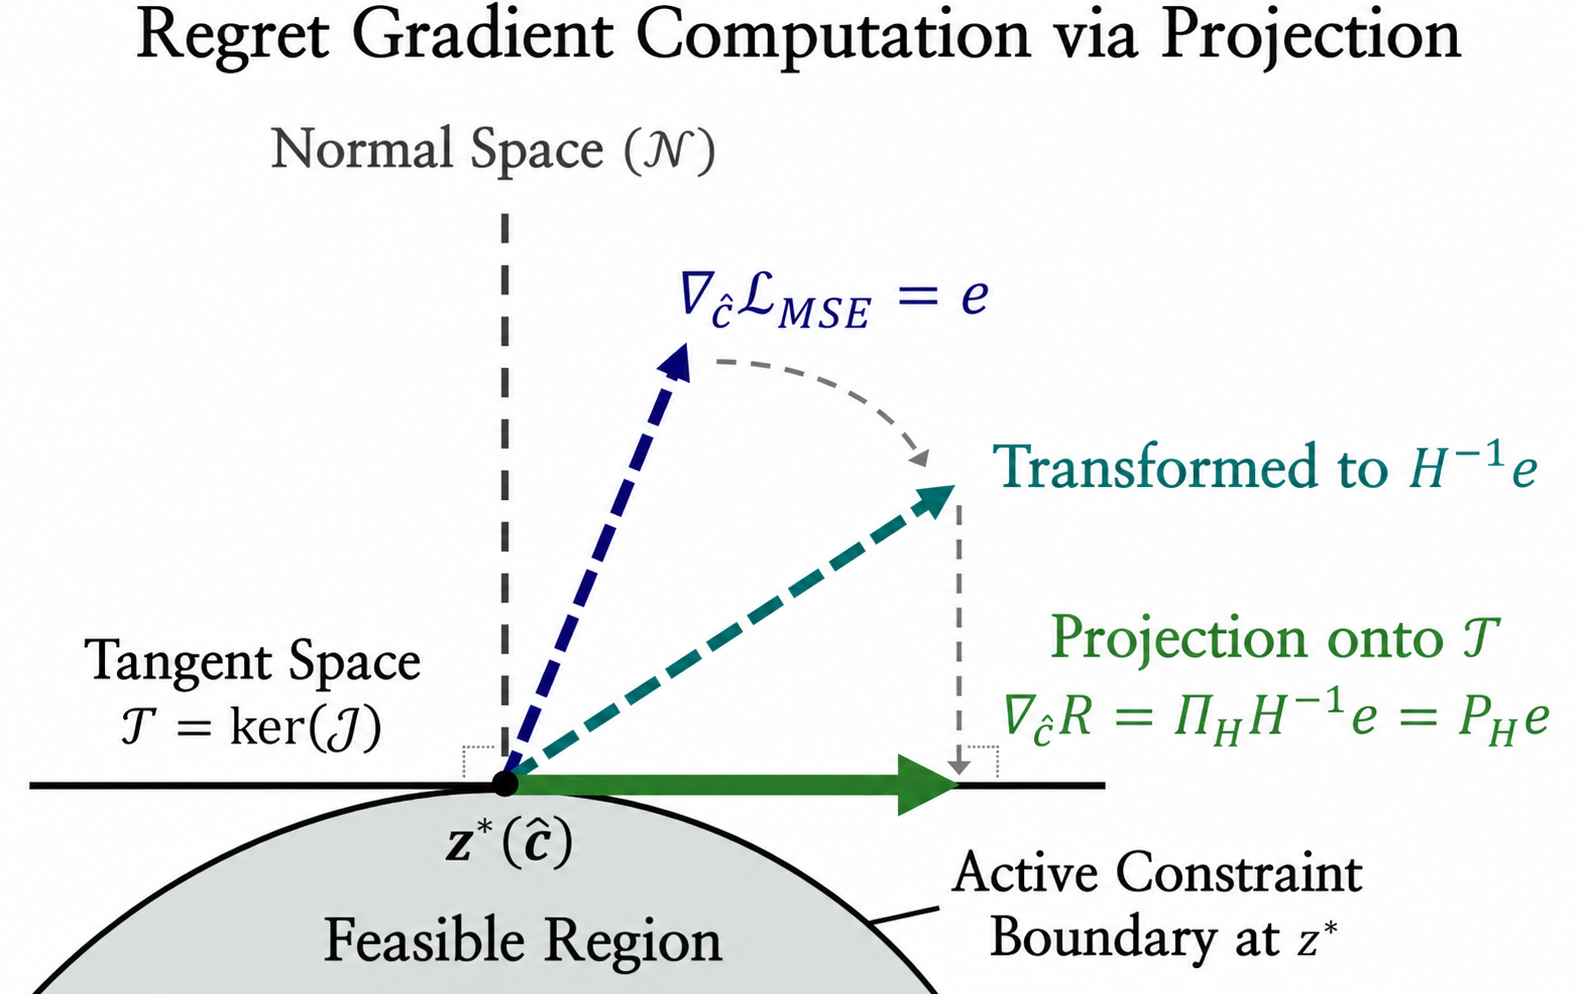
\includegraphics[width=0.78\linewidth,height=0.56\textheight,keepaspectratio]{figures/regret_gradient_projection.png}
    \end{center}


\end{frame}

%------------------------------------------------

\section{Computing the Projected-Error Gradient}

\begin{frame}[plain,noframenumbering]
    \sectionpage
\end{frame}

\begin{frame}{General Framework of PEAR}
    \begin{columns}[T,onlytextwidth]
        \begin{column}{0.40\textwidth}
            \small
            From last section,
            \[
                \nabla_{\hat{\vc}}R(\hat{\vc};\vc)
                =\mP_H(\hat{\vc}-\vc).
            \]

            The general update is still the classic first-order gradient descent:
            {\footnotesize
            \begin{equation}
                \begin{aligned}
                    \frac{dR}{d\vtheta}
                    &=\frac{\partial\hat{\vc}^{\top}}{\partial\vtheta}
                      \nabla_{\hat{\vc}}R(\hat{\vc};\vc)\\
                    &=\left(\frac{\partial\hat{\vc}}{\partial\vtheta}\right)^{\top}
                      \mP_H(\hat{\vc}-\vc).
                \end{aligned}
            \end{equation}}

            The key is to compute
            \[
                \vg:=\nabla_{\hat{\vc}}R(\hat{\vc};\vc)
                =\mP_H(\hat{\vc}-\vc)
            \]
            efficiently, rather than forming
            $\mP_H\in\R^{n\times n}$ explicitly.
        \end{column}

        \begin{column}{0.58\textwidth}
            {\fontsize{7.2}{8.3}\selectfont
            \textbf{Algorithm 1 PEAR: Projected Error as Regret-gradient}\par
            \vspace{0.1em}
            \hrule
            \vspace{0.25em}

            {\fontsize{5.9}{7}\selectfont
            \begin{tabular}{@{}p{0.12\linewidth}p{0.83\linewidth}@{}}
                \textbf{Input:} & Predicted costs $\hat{\vc}=f_{\vtheta}(\vx)$,
                true costs $\vc$, problem data $(\mA,\vb,\mG,\vh)$\\
                \textbf{Input:} & Hessian $\mH=\nabla^2\phi(\vz^*)$
                (or $\mH=\lambda\mI$ for LP), injection strength $\beta\in[0,1]$\\
                \textbf{Output:} & Gradient signal
                $\vg=\nabla_{\hat{\vc}}R(\hat{\vc};\vc)$
            \end{tabular}}

            \vspace{0.25em}
            \hrule
            \vspace{0.25em}

            {\fontsize{5.9}{7}\selectfont
            \begin{tabular}{@{}r@{\hspace{0.35em}}p{0.88\linewidth}@{}}
                1: & \textbf{// Forward: Active-Set Detection}\\
                2: & Solve (1) with cost $\hat{\vc}$ to obtain primal-dual pair $(\vz^*,\vy^*)$\\
                3: & Identify active set $\mathcal A$ via complementary slackness (16)\\
                4: & Form active constraint Jacobian
                     $\mJ\leftarrow \left[\mA^\top , \mG_{\mathcal A}^\top\right]^\top$\\
                5: & \textbf{// Backward: Compute $\mP_H\ve$ via Reduced System}\\
                6: & Compute prediction error $\ve\leftarrow\hat{\vc}-\vc$\\
                7: & Compute $\vx\leftarrow\mH^{-1}\ve$ and $\vr\leftarrow\mJ\vx$\\
                8: & Solve $(\mJ\mH^{-1}\mJ^\top)\vv=\vr$ for $\vv$\\
                9: & Compute projected gradient
                     $\vg\leftarrow\vx-\mH^{-1}\mJ^\top\vv$\\
                10: & \textbf{// Optional: Normal injection for LP}\\
                11: & \textbf{if} $\beta>0$ \textbf{then}\\
                12: & Compute normal component
                      $\vn\leftarrow\mH^{-1}\mJ^\top\vv$\\
                13: & $\vg\leftarrow\vg+
                      \beta\cdot\frac{\lVert\vg\rVert}{\lVert\vn\rVert}\cdot\vn$\\
                14: & \textbf{end if}\\
                15: & \textbf{return} $\vg$
            \end{tabular}}

            \vspace{0.25em}
            \hrule
            }
        \end{column}
    \end{columns}
\end{frame}

\begin{frame}{Forward Pass: Active-Set Detection}

    Not too much theory.

    \begin{enumerate}
        \item First, use a solver \texttt{OSQP} to solve the optimization problem $\vz^*(\hat{\vc}) \in \arg\min_{\vz} \phi(\vz) + \hat{\vc}^\top \vz$ s.t. $\mA \vz = \vb, \mG \vz \leq \vh$, and obtain the primal-dual pair $(\vz^*,\vy^*)$.
        \item Then, identify the active set $\mathcal{A}(\hat{\vc})$ via complementary slackness: $\mathcal{A}(\hat{\vc}) = \{i : (\mG \vz^*(\hat{\vc}))_i = \evh_i\}$.
        \item Finally, form the active constraint Jacobian $\mJ = [\mA^\top , \mG_{\mathcal{A}}^\top]^\top$.

    \end{enumerate}

\end{frame}

\begin{frame}[allowframebreaks]{Backward Pass: Efficient Gradient Computation}

    Recall, given a perterbation in predicted cost $d\hat{\vc}$, the corresponding perturbation in optimal solution is $d\vz = -\mP_H d\hat{\vc}$. Now, specify the perturbation value as the prediction error
    \begin{equation}\label{eq:ve_perturbation}
        d\hat{\vc} \leftarrow - \ve .
    \end{equation}

    Plug in this specific perturbation into the sensitivity KKT system (\eqref{eq:reduced_kkt_linear}) gives:
    \begin{equation}\label{eq:reduced_kkt_linear_ve}
        \begin{bmatrix}
            \mH & \mJ^\top\\
            \mJ & 0
        \end{bmatrix}
        \begin{bmatrix}
            d\vz\\
            d\vy
        \end{bmatrix}
        =
        \begin{bmatrix}
            \ve\\
            0
        \end{bmatrix}
    \end{equation}
    Computing \eqref{eq:reduced_kkt_linear_ve} gives:
    \begin{equation}\label{eq:dz_dy_ve}
        d\vz =\underbrace{\mH^{-1} \ve}_{\text{free movement}} - \underbrace{\mH^{-1} \mJ^\top d\vy}_{\text{constraint correction}}, \qquad \underbrace{\mJ d\vz}_{\text{active constraint}} = 0 .
    \end{equation}
    Solving this linear system gives the projected prediction error $d\vz = \mP_H \ve$.

    \break

    It solves with some tricks as follows. Combining the two gives the reduced system:
    \begin{equation}
        \boxed{
            \mJ \mH^{-1} \mJ^\top d\vy = \mJ \mH^{-1} \ve
        }
    \end{equation}
    To simplify notation, $\vx:= \mH^{-1} \ve \in \R^n$, $\vr := \mJ \vx \in \R^k$, and $\vv := d\vy \in \R^k$. Then the reduced system (only involves $k$ variables) is
    \begin{equation}
            \mJ \mH^{-1} \mJ^\top \vv = \vr
    \end{equation}
    Then once $\vv = d\vy$ is solved, recall that $\vg = \mP_H \ve$ (\eqref{eq:regret_gradient}), $d\vz = - \mP_H d\hat{\vc}$ (\eqref{eq:dz_dhatc_final}), and $d\hat{\vc} = -\ve$ (\eqref{eq:ve_perturbation}). These three equations give $\vg = d\vz$. Further by $d\vz = \vx - \mH^{-1} \mJ^\top \vv$ (\eqref{eq:dz_dy_ve}), it gives
    \begin{equation}
        \boxed{
            \vg = d\vz = \vx - \mH^{-1} \mJ^\top \vv
        }
    \end{equation}


\end{frame}

%------------------------------------------------

\begin{frame}{References}
    \footnotesize
    \bibliography{reference.bib}
    \bibliographystyle{apalike}
\end{frame}

%----------------------------------------------------------------------------------------

\end{document}
